\begin{figure}[hb]
	\centering
	\begin{tikzpicture}[scale=\textwidth/\paperwidth]
		\begin{scope}[>=latex, node distance=1, align=center, transform shape]
			\node	(aux1)	[]	{};
			\node[core,	minimum height=95]
					(mis)	[left=of aux1,anchor=north east]	{MIS};
			\node[core]	(ram)	[right=of aux1,anchor=north west, text width=30]	{16 kB RAM};
			\node[perif,text width=60]
					(xcvr)	[left=of mis]	{Transceptor USB};
			\node[interior,	minimum size=60, text width=50]
					(uc)	[above=of aux1]	{8051 Mejorado};			
			\node[perif,
			node distance=2.9]
				(pll)	[left=of uc]	{PLL};		
			\node	(aux2)	[right=of ram.south]{};				
			\node[core,	text width=120]
				(bus)	[right=of aux2,rotate=90,anchor=north west]	{Bus de datos y direcciones};		
			\node[perif]	(i2c)	[right=of bus.south east,anchor=north west]	{I2C};
			\node[perif,text width=30]
				(gpif)	[right=of bus.south west,anchor=south west] {GPIF};
			\node[perif,text width=40]
				(fifo)	[below=of gpif]	{4 kB FIFO};
			\node	(aux3)	[right=of fifo]	{};
			\node	(aux5) 	[left=of ram] {};
			\draw[<->]	(mis) -- (xcvr);
			\draw[<->]	(ram) -- (ram -| mis.east);
			\draw[<->]	(fifo) -- (fifo -| mis.east);
			\draw[<->]	(ram) to (ram -| bus.north);
			\draw[<->]	(uc) to (uc -| bus.north);
			\draw[<-]	(xcvr) to (xcvr |- pll.south);
			\draw[->]	(pll) to (uc);
			\draw[<->]	(i2c) to (i2c -| bus.south);
			\draw[<->]	(gpif) to (gpif -| bus.south);
			\draw[]		(fifo) -| (aux5.center);
		\end{scope}
	
		\begin{scope}[on background layer]
			\node[contenedor] (fx2) [fit=(pll)(xcvr)(uc)(bus)(mis)(ram)(fifo)(gpif)(i2c)(aux3)]{};
		\end{scope}
		
		\begin{scope}[transform shape,>=latex]
			\node[text width=40,align=center]	(xtal)	[left=of pll]{Xtal \SI{24}{\mega\hertz}};
			\node	(host)	[left=3of xcvr]	{PC};
			\draw[<->,ultra thick] (host) -- node [above,text width=70,midway,align=center]{Comunicación USB} (xcvr);
			\draw[->] (xtal) to (pll);
			\draw[<->,ultra thick] (bus.240) -- node [above,align=center,text width=80] {Datos, direcciones y entradas adicionales}(bus.240 -| fx2.east);
			\draw[<->,thick] (gpif) to (gpif -| fx2.east);
			\draw[<->,thick] (fifo) to (fifo -| fx2.east);
			\draw[<->,thick] (i2c) to (i2c -| fx2.east);
		\end{scope}
	\end{tikzpicture}
	%		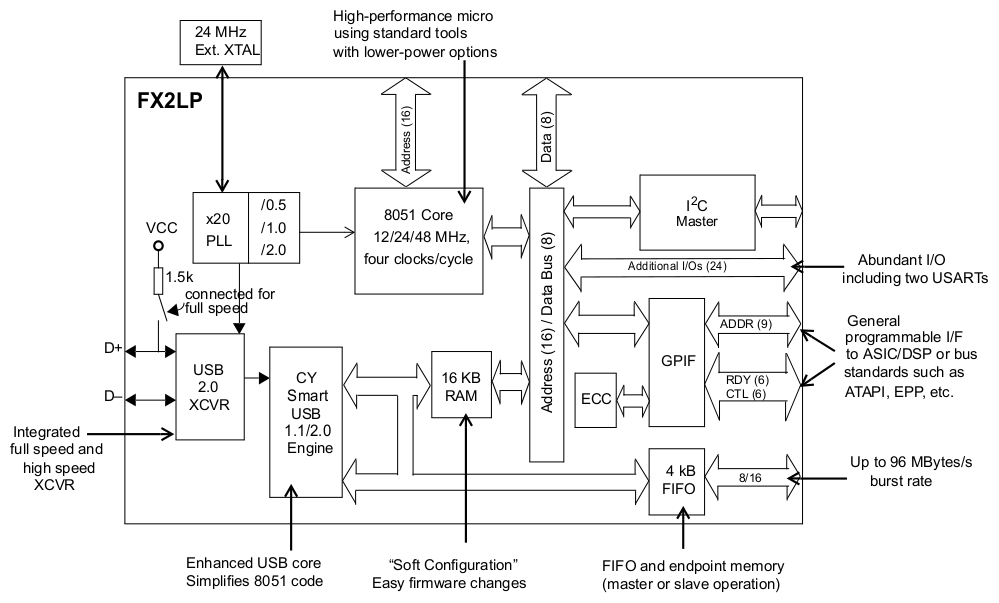
\includegraphics[width=.7\textwidth]{arqfx2lp.png}
	%		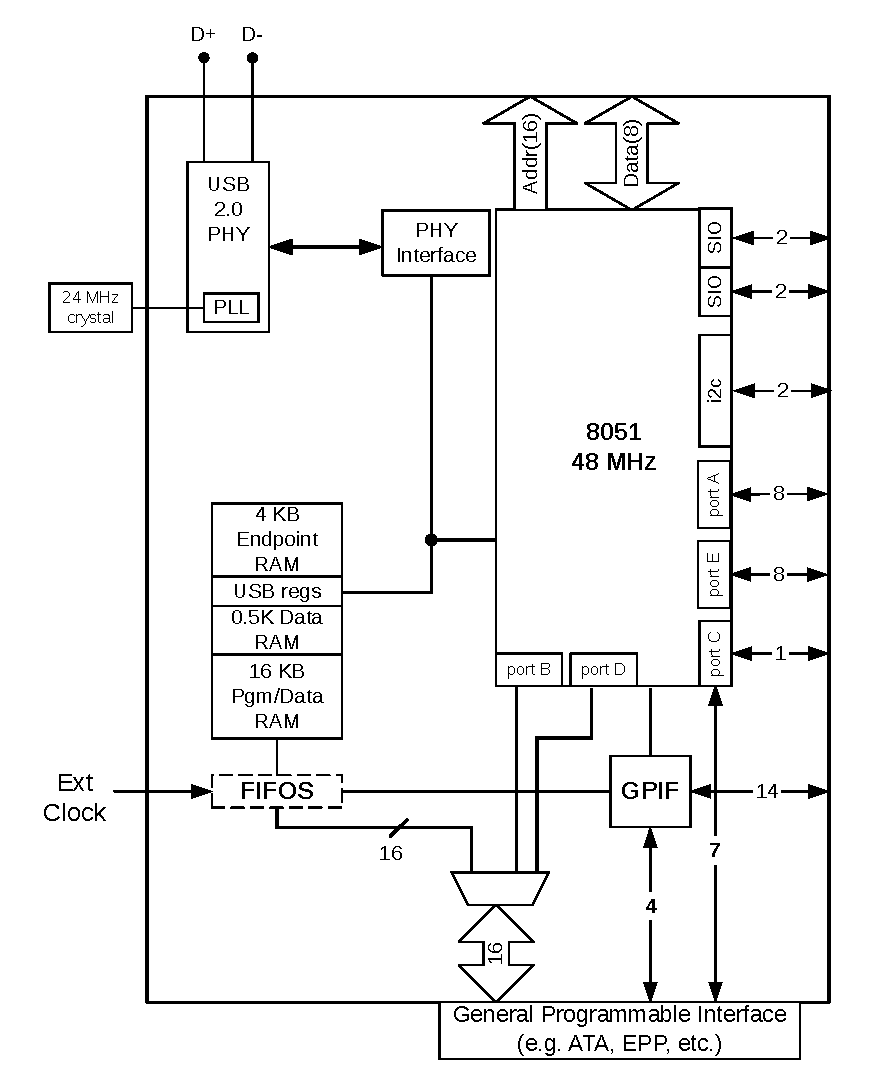
\includegraphics[width=.55\textwidth]{arq.eps}
	\caption{Arquitectura FX2LP} 
	\label{arqEzUSB}
\end{figure}

El núcleo del kit de desarrollo CY3684 es el controlador EZ-USB FX2LP. La serie de controladores FX2LP se caracteriza por brindar una conexión USB 2.0 de alta velocidad y bajo consumo energético. Está diseñada, preferentemente más no exclusivamente, para periféricos que se alimentan a baterías y poseen una autonomía energética limitada.

La arquitectura de controlador FX2LP, tal como se presenta en la Figura \ref{arqEzUSB}, integra un controlador USB completo, es decir, incluye un transceptor USB, un Motor de Interfaz Serie (MIS) y buffers configurables para datos. Incorpora también una versión del microcontrolador ($\mu$C) Intel MCS-51, más conocido como el $\mu$C 8051, que contiene registros y funciones adicionales orientadas a mejorar el rendimiento de la comunicación USB y memoria RAM de \SI{16}{\kilo\byte} de capacidad, para almacenar programas y datos. 
%Cypress agrega, como interfaz programable hacia los periféricos, una memoria tipo FIFO (\(First In First Out\); Primero Entrado, Primero Salido) con una capacidad de \SI{4}{\kilo\byte} que es operada en modo esclavo (es decir, necesita un dispositivo que le provea la lógica para operar) y destinada a almacenar datos de la comunicación, una interfaz de propósito general (GPIF) y un puerto I$^2$C. Además posee un PLL con divisor configurable a través del cual provee las señales de reloj adecuadas para el correcto funcionamiento del sistema.%\\
El modelo del flujo de datos posee dos extremos entre las cuales el controlador cumple el rol de interfaz. Estos extremos son la PC y el FPGA respectivamente. El controlador necesita, entonces, poder comunicarse tanto con el Host como con los periféricos. Para este propósito, Cypress agrega al circuito integrado del controlador dos puertos USART ((acrónimo de Transmisión y Recepción Asíncrona en Serie Universal, en inglés)), una interfaz de propósito general (GPIF), un puerto I$^2$C y una memoria FIFO (\(First In First Out\); Primero Entrado, Primero Salido).

La GPIF está pensada principalmente para poder utilizar sistemas que deban ser comandados en forma externa, como por ejemplo un registro de desplazamiento. Por su parte, la memoria FIFO posee \SI{4}{\kilo\byte} de capacidad reservados para almacenar los datos que se intercambian y se destina a aquellos sistemas que pueden proveer las señales de control, aunque también puede ser comandada por el GPIF. Con estas interfaces se posibilita la conexión con casi cualquier dispositivo, ya sea estandarizado (ATA, PCMCIA, EPP, etc) o personalizable (DSP, FPGA, $\mu$C);

%El usuario puede trasmitir datos desde y hacia el Host a través del mismo puerto USB. Sin embargo, también posee dos puertos USART ((acrónimo de Transmisión y Recepción Asíncrona en Serie Universal, en inglés)) que permiten comunicarse con la PC y facilitan en gran medida la tarea de depuración del desarrollo.

%En cuanto a la interfaz con uno o mas periféricos, el controlador posee un puerto $I^2C$, una interfaz de propósito general (GPIF), para sistemas que necesitan ser comandados en forma externa; y una interfaz con memorias FIFO esclavas, a través de las cuales se puede conectar sistemas que cumplen un rol activo en el envío y recepción de información. Estas tres interfaces posibilitan la conexión de dispositivos que poseen tanto puertos estandarizados (ATA, PCMCIA, EPP, etc.), cómo personalizables (DSP, FPGA, microcontroladores, etc).

%Variante 1
 
%El usuario puede trasmitir datos desde y hacia el anfitrión a través del mismo puerto USB, o bien via RS-232. Para comunicarse con sistemas periféricos se puede aprovechar el puerto $I^2C$, la interfaz de propósito general, que actúa como maestro y a la cual se le puede acoplar un periférico esclavo, y/o las memorias FIFO en modo esclavo que puede ser conectada a un sistema maestro. Esto brinda muchas alternativas, desde la conexión a puertos estandar, como ser ATA, PCMCIA, EPP, etc. o también la conexión de dispositivos tales como DSP's y FPGA's.\\
%\textbf{\hl{variante 1}}
%\hl{El usuario puede trasmitir datos desde y hacia el anfitrion a traves del mismo puerto USB, o bien via RS-232. Para comunicarse con sistemas perifericos se puede aprovechar el puerto $I^2C$, la interfaz de proposito general, que actua como maestro y a la cual se le puede acoplar un periferico esclavo, y/o las memorias FIFO en modo esclavo que puede ser conectada a un sistema maestro. Esto brinda muchas alternativas de conexion, desde puertos estandar, como ser ATA, PCMCIA, EPP, etc. hasta dispositivos personalizables como DSP's y FPGA's}.%\\

%variante 2
%El flujo de datos posee dos puntas entre las cuales el controlador hace de nexo. Para ello necesita poder comunicarse tanto con el \host como con los periféricos.\\
%
%El intercambio de información con el \host se lleva a cabo a través del mismo puerto USB, objetivo principal de este trabajo. Sin embargo, también posee dos puertos UART que facilitan en gran medida la tarea de depuración del desarrollo.\\
%
%En cuanto a la interfaz con uno o más periféricos, el controlador posee un puerto $I^2C$, una interfaz de propósito general (GPIF), para sistemas que necesitan ser comandados en forma externa; y una interfaz con memorias FIFO esclavas, a través de las cuales se puede conectar sistemas que cumplen un rol activo en el envío y recepción de información.\\

%\textbf{\hl{variante 2}}
%
%\hl{El flujo de datos posee dos puntas (una PC y un FPGA) entre las cuales el controlador cumple el rol de interfaz. Para ello necesita poder comunicarse tanto con el host como con los perifericos.}%\\
%
%\hl{El intercambio de informacion con el HOST se lleva a cabo a traves del mismo puerto USB, objetivo principal de este trabajo. Sin embargo, tambien posee dos puertos UART que facilitan en gran medida la tarea de depuracion del desarrollo.}%\\
%
%\hl{En cuanto a la interfaz con uno o mas perifericos, el controlador posee un puerto $I^2C$, una interfaz de proposito general (GPIF), para sistemas que necesitan ser comandados en forma externa; y una interfaz con memorias FIFO esclavas, a traves de las cuales se puede conectar sistemas que cumplen un rol activo en el envio y recepcion de informacion.}%\\

Bajo el criterio de este autor, el componente de mayor trascendencia en el funcionamiento del controlador FX2LP es el $\mu$C 8051. Es este componente el encargado de configurar los bloques programables y de inicializar todos los registros que determinan la forma en la que el sistema funciona: la frecuencia de trabajo, la gestión de las memorias y el modo en que fluyen los datos son algunas de las tareas que configura el $\mu$C. El firmware es escrito en lenguaje C para microcontroladores. 

La estructura de la interfaz implementada en este trabajo utiliza la memoria FIFO en modo esclavo, es decir, la memoria responde a señales que proporciona un maestro externo sintetizado en un FPGA. Se escogió la frecuencia de funcionamiento del PLL y se configuraron los extremos que intervienen en la comunicación USB y el modo de funcionamiento, por lo que a continuación se explicitan los detalles referidos a la configuración realizada, con lo que se busca aclarar el funcionamiento y que el lector comprenda los fundamentos de las configuraciones que se plasman en el código del firmware.

\subsection{Microcontrolador Cypress 8051 Mejorado}
	Las tareas que ejecuta el controlador FX2LP son llevadas a cabo por un microcontrolador incorporado al circuito integrado. Dicho $\mu$C es una modificación del 8051 desarrollado por Intel, para que sea más veloz en sus tiempos de ejecución y mejore el desempeño del $\mu$C cómo interfaz, mediante la incorporación de registros especiales adicionales.  De esta forma, la manera a través de la cuál el desarrollador elabora la configuración del controlador, es a través de la programación de este $\mu$C 8051.
	
	Para elaborar el firmware que ejecuta el controlador FX2LP, se desarrolló un programa en C para microcontroladores y se compiló mediante el compilador C51 de Keil, a través del entorno de desarrollo integrado Keil $\mu$Vision.
	
	Cypress provee, dentro del kit de desarrollo CY3684, un conjunto de archivos que contienen código base sobre el cual el desarrollador implementa la configuración. Este conjunto de archivos es denominado framework, el cual posee, entre otras cosas, encabezados con definiciones de macros, constantes, registros, tipos de datos y declaración de funciones prototipo. También incorpora algunas funciones precompiladas para utilizar los periféricos que contiene la placa de desarrollo.
	
	\begin{figure}[ht]
		\centering
		\begin{tikzpicture}[scale=.75\textwidth/\paperwidth]
			\begin{scope}[transform shape,node distance=1,>=latex]
				\node[mealy]	(start)	[]	{Iniciar: Reset \\ \verb|main();|};
				\node[moore]	(init)	[below=of start]	{Inicia Variables de Estado}
				edge[<-,thick] (start);
				\node[moore]	(us1)	[below=of init]		{\verb|TD_Init();|}
				edge[<-,thick]	(init);
				\node[moore]	(EI)	[below=of us1]	{Habilita\\Interrupciones}
				edge[<-,thick](us1);
				\node[node distance=0.7]			(aux1)	[below=of EI] 	{};
				\draw[<-,thick](aux1.base) to (EI);
				\node[moore,node distance=.5]	(poll)	[below=of aux1]	{\verb|TD_Poll();|}
				edge[<-,thick](aux1.base);
				\node[ask]		(pr1)	[below=of poll]	{Paquete de Setup}
				edge[<-,thick](poll);
				\node[moore]	(setup)	[right=of pr1]	{\verb|SetupComand();|};
				\draw[->,thick] (setup) |- (aux1.base);
				\node[]			(aux2)	[below=of pr1]	{};
				\draw[->,thick]	(pr1) -- node[above,near start]{Si} (setup);
				\draw[thick]	(pr1) -- node[left,near start]{No}	(aux2.base);
				\node[node distance=2.5](aux3)	[left=of aux2] {};
				\draw[thick]	(aux2.base) -- (aux3.base);
				\draw[->,thick]	(aux3.base)	|-	(aux1.base);
			\end{scope}
		\end{tikzpicture}
		\caption{Diagrama en bloques del firmware que ejecuta el $\mu$C de la interfaz}
		\label{int:fw}
	\end{figure}
	
	La Figura \ref{int:fw} muestra un diagrama de flujo del firmware que se desarrolló en el presente trabajo. El mismo se elaboró utilizando la estructura propuesta por Cypress para el desarrollo de la comunicación que se implementó. Se puede observar que al inicio del programa se inicializan variables de estado que corresponden a una máquina de estados, desarrollada por Cypress, que ejecuta las tareas de la comunicación USB.
	
	Luego, se invoca una función llamada \verb|TD_Init()|. Esta es la función a través de la cual se implementa la configuración que se desarrolló en este trabjo. En las secciones siguientes se profundiza cada uno de los bloques que intervienen.
	
	Una vez configurado el funcionamiento del controlador, se habilitan las interrupciones, lo que da lugar a que todas los bloques del circuito integrado puedan funcionar e intercambiar información. Seguidamente, el programa entra en un lazo infinito, donde en primer lugar ejecuta la función \verb|TD_Poll()|, en la cual el desarrollador programa las tareas que ejecuta el controlador durante la rutina de funcionamiento. Como segundo paso, el controlador chequea si arribó desde el Host una transferencia de control cuyo PID indique Setup. En caso afirmativo, ejecuta lo solicitado por el Host. En caso contrario, vuelve a ejecutar la función \verb|TD_Poll()|.
	
%	Keil μVision es un entorno de desarrollo integrado (IDE). Se entiende por IDE a un software
%	que integra en un entorno gráfico las herramientas que permiten elaborar un programa que
%	ejecutará un procesador, desde la escritura del algoritmo en uno o más lenguajes, su compilación,
%	las pruebas y el depurado.
%	El programa utilizado posee, entre otras cosas, editor de textos con atajos de teclado,
%	comandos que aceleran la escritura de código y resaltado de palabras claves para diferentes
%	lenguajes de programación, navegador de archivos. También ejecuta, con solo un click, el
%	compilador con la sintaxis correcta, y posee un depurador que, a través de un intérprete, permite
%	ir ejecutando el código lı́nea por lı́nea o en bloques.
%	Para realizar un programa en este entorno, Cypress provee, junto con su framework, un
%	proyecto vacı́o que puede ser copiado y pegado. Sin embargo, se puede realizar la configuración
%	manual. Las instrucciones de este procedimiento se ubican en el Apéndice ??.
%	En cuanto al compilador se refiere, el utilizado es C51. Éste es un programa que otorga
%	un archivo hexadecimal con un código que será ejecutado por microcontroladores que estén
%	implementados con la misma estructura que un Intel 8051, cómo lo es el microcontrolador que
%	posee el FX2LP.
\subsection{Frecuencia de trabajo del sistema}
	Como se menciona en la sección anterior, la configuración principal del sistema se realiza a través de la función \verb|TD_Init()|. El primer módulo configurado es el PLL ({\it Phase-Locked Loop}). Un PLL es un lazo de servocontrol cuyo parámetro controlado es la fase de una réplica, generada en forma local, de una señal de entrada\cite{Sklar2001}. En otras palabras, permite obtener dos señales iguales a través de un detector de fase. Si se incorpora un contador entre la señal generada y la entrada del comparador de fase, la señal generada tendrá una frecuencia igual al producto de la entrada por el recorrido del contador. Si, en cambio, se coloca el contador a la salida del PLL, la frecuencia puede ser dividida. Así, es posible obtener señales de frecuencia modificable.

	El PLL incorporado en el controlador permite elevar la frecuencia de un cristal de \SI{24}{\mega\hertz} hasta los \SI{480}{\mega\hertz} que necesita el transceptor USB para el cumplimiento de la norma USB. A su vez, a través de un divisor de frecuencias, permite seleccionar diferentes frecuencias de trabajo del $\mu$C 8051, entre \si{12}, \si{24} o \SI{48}{\mega\hertz}.
	
	A través de los bits especiales CLKSPD[1:0] del registro de Control y Estado de CPU (CPUCS). En la implementación realizada, se seleccionó la frecuencia de trabajo del $\mu$C a \SI{48}{\mega\hertz}.
	
	\begin{lstlisting}[language=C,backgroundcolor=\color{gray!30}]
	//CPUCS - Registro de Control y Estado del CPU
	//	CLKSPD[1:0] -> "00" => 12 MHz
	//				-> "01" => 24 MHz
	//				-> "10" => 48 MHz
	CPUCS = ((CPUCS & ~bmCLKSPD) | bmCLKSPD1); // 48 MHz
	\end{lstlisting}	

\subsection{Memoria FIFO}
	El controlador FX2LP posee una sección especial de memoria destinada al almacenamiento de los datos que fluyen desde cada uno de los extremos de la comunicación. A esta memoria pueden acceder tanto los componentes del propio controlador, como también los periféricos que desean comunicarse a través de él. Desde el punto de vista de la electrónica digital, cada uno de los componentes que acceden a esta memoria pueden tener diferentes fuentes de señal de reloj. Para salvar los inconvenientes que puede acarrear el uso de sistemas con fuentes de reloj independientes, esta porción de memoria reservada es de tipo FIFO. Debido a que se puede acceder a estas memorias FIFO tanto desde el interior de controlador FX2LP, como desde el exterior, deben ser configuradas en ambos sentidos.
	
	La memoria FIFO puede ser programada y configurada de diferentes formas, en función de los requerimientos sistemas periféricos acoplados a ella. Cada uno de los periféricos conectados a la memoria FIFO se denomina extremo o EP\footnote{EP es una abreviación del término inglés {\it endpoint}, que significa ``Extremo''. Esto quiere decir que cada uno de los periféricos conectados a la memoria FIFO es un extremo de la comunicación.}. Las características a configurar son el tamaño (\si{64}, \si{512} o \SI{1024}{\byte}), la cantidad de bloques o partes en que se divide la memoria (puede estar dividida hasta en 4 extremos) y la cantidad de buffers de datos utilizados para almacenar los datos de cada bloque de memoria.
	
	Los buffers son porciones de memoria físicamente separadas pero que, en la operación, el controlador puede intercambiar de forma tal que se acceda a ellos a través de una misma dirección de memoria. El uso de buffers múltiples implica que un EP utiliza más de un buffer. Los buffers múltiples poseen la función de evitar la congestión de datos. Con doble buffer, un periférico coloca o extrae datos del buffer de un EP, mientras el $\mu$C, utiliza otro del mismo EP. La selección del buffer donde cada componente escribe y/o lee los datos lo asigna e intercambia la interfaz en forma automática. Se pueden configurar también un triple o cuádruple buffer, lo que agrega sendas porciones de memoria extra a la reserva. De esta forma, se le otorga al sistema, en forma simultánea, gran capacidad de datos y ancho de banda.
	
	En este desarrollo, se configuró la memoria FIFO con dos EP. El EP2\footnote{EP con dirección 2.}, es un EP de entrada (envía datos al Host). Requiere una gran cantidad de datos, debido a que será por donde los sensores transmitirán todos los datos que adquieran. Además, es necesario que posea una buena cantidad de almacenamiento de datos y que estos datos sean enviados de la forma más rápida posible. Por tanto, el EP2 se configuró con dos buffers de \SI{1024}{\byte}, para que efectúe transferencias isócronas.
	
	Por su parte, se configura el EP8 como EP de salida (recibe datos desde el Host). Este EP se utiliza para recibir la configuración de los sensores, que se espera que sea de menor cantidad y más distanciada en el tiempo que los datos adquiridos. Se configuró, entonces, con dos buffers de \SI{512}{\byte} para transferencias en masa.
	
	Debido a que la memoria FIFO cumple el rol de interfaz entre los periféricos y el módulo del controlador FX2LP que efectúa las tareas propias de la comunicación USB, la configuración de dicha memoria se efectúa por separado, conteniendo información relevante a cada etapa de la comunicación.
	
\subsubsection{Interfaz hacia los periféricos}
	Cypress provee varias interfaces para comunicar el controlador hacia los periféricos. I$^2$C y UART son dos posibilidades, aunque poseen un ancho de banda muy limitado. La interfaz que opera con mayor ancho de banda es la memoria FIFO. Esta puede ser utilizadas en modo esclavo, es decir, que un sistema externo comande la lectura y la escritura de datos en ellas, o bien, a través de la interfaz GPIO, puede ser comandada por el $\mu$C 8051. La implementación que se realiza en el desarrollo de la comunicación utiliza la memoria FIFO en modo esclavo.
	
	La frecuencia de funcionamiento de estas interfaz es independiente del reloj del sistema. Puede ser configurado para usar una señal de reloj interna de \si{30} o \SI{48}{\mega\hertz}, propia de la interfaz, o bien, ser provista por un sistema externo al controlador. También, es importante indicarle al controlador si la interfaz funcionará en modo asíncrono. Todos estos parámetros son configurados a través del registro Configuración de Interfaz (IFCONFIG).
	
	La configuración que se realizó en esta implementación, utiliza el reloj interno de la interfaz, corriendo a \SI{48}{\mega\hertz}. Además, se indica que las memorias FIFO esclavas son utilizadas en modo asincrónico. Dicha configuración se plasma en las siguientes líneas de código:
	
	\begin{lstlisting}[language=C,backgroundcolor=\color{gray!30}]
	//IFCONFIG - Registro de Configuración de la Interfaz
	//	b7 	   -> fuente de reloj: '1' interna, '0' externa
	//	b6 	   -> frec: '1' 48 Mhz, '0' 30 MHz
	//	b3 	   -> asinc: '1' asíncrono
	//	b[1:0] -> modo de interfaz: "11" FIFO esclava
	IFCONFIG = 0xCB;
	SYNCDELAY;
	\end{lstlisting}

	El controlador FX2LP posee cuatro puertos que emiten señales del estado de las memorias FIFO. Estos puertos pueden ser programados para que indiquen si una porción particular de memoria se encuentra vacía, llena o si sobrepasa un nivel programable de datos. También pueden ser configurados para que indiquen el estado completo (vacío, lleno y el nivel programable) de la porción de memoria activa. Cada porción de memoria se activa a través de dos puertos de dirección, comandados por un sistema externo al controlador FX2LP.
	
	Para la comunicación desarrollada, solo son importantes las señales que indican cuando el puerto que se corresponde al EP8 está vacío y el que señala al EP2 está lleno. Si bien no son necesarias, por completitud, también se configuraron las señales EP2 vacío y EP8 lleno. Cada uno de los puertos de señal se denominan A, B, C y D y se configuran por pares a través de los registros PINFLAGSAB y PINFLAGSCD, de la forma en que se muestra a continuación.
	
	\begin{lstlisting}[language=C,backgroundcolor=\color{gray!30}]
	PINFLAGSAB = 0xBC;	// FLAGA <- EP2 Full Flag
						// FLAGD <- EP2 Empty Flag
	SYNCDELAY;
	PINFLAGSCD = 0x8F;	// FLAGC <- EP8 Full Flag
						// FLAGB <- EP8 Empty Flag
	\end{lstlisting}
	
	
\subsubsection{Interfaz hacia el módulo de comunicación USB}
	Desde el extremo interno del controlador FX2LP, la memoria FIFO se conecta al Motor de Interfaz Serial (MIS). El MIS es un módulo que se encarga de tomar datos en paralelo y convertilos en una secuencia seriada. Para cumplir con la norma USB, el MIS debe ser capaz de empaquetar, enviar, recibir y desempaquetar toda la información, así como leer los tokens que emite el host, calcular y corroborar los códigos cíclicos de detección de errores y todo lo relacionado al protocolo propiamente dicho. Luego, el transceptor USB efectúa las tareas de codificación y decodificación de los mensajes transmitidos a través del bus.
	
	Para la configuración, es necesario indicarle al controlador FX2LP el funcionamiento que tendrá cada uno de los EP. Los parámetros programables son: si está activo o no, el sentido de la comunicación (sea hacia o desde el Host), el tipo de transferencia, el tamaño de la misma y la cantidad de buffers múltiples que se utilizan. En el desarrollo que se presenta se configura el EP2 como entrada de \SI{1024}{\byte} con dos buffers y el EP8 como salida con dos buffers de \SI{512}{\byte}. También se configura el EP1 con un buffer de \SI{64}{\byte} como entrada y otro igual como salida, ya que viene implementado en una memoria separada dentro del circuito integrado FX2LP y no interfiere con el desempeño pretendido en este trabajo. Los otros EP válidos (EP4 y EP6) no se utilizan, con el objetivo de maximizar la memoria disponible para los datos útiles. De esta forma, la configuración se realiza a través de la siguiente línea de código:
	
	\begin{lstlisting}[language=C,backgroundcolor=\color{gray!30}]
	//EPxCFG - Registros de configuración de extremos
	//	b7 	   -> '1' EP activo
	//	b6 	   -> dir: '0' salida, '1' entrada
	//	b[5:4] -> tipo: "01" => isocronico
	//					"10" => masa
	//					"11" => interrupción
	//	b3 	   -> tamaño: '0' 512 bytes, '1' 1024 bytes
	//	b[1:0] -> buffer: 	"00" => x4
	//						"10" => x2
	//						"11" => x3
	EP1OUTCFG = 0xA0;
	SYNCDELAY;
	EP1INCFG = 0xA0;
	SYNCDELAY;
	// dir:entrada, tipo:isoc, tam:1024, x3
	EP2CFG = 0xDB;
	SYNCDELAY;
	EP4CFG = 0x7F; //Inactivo
	SYNCDELAY;
	EP6CFG = 0x7F; //Inactivo
	SYNCDELAY;
	// dir:salida, tipo:masa, tam:512, x2
	EP8CFG = 0xA2; 
	SYNCDELAY;
	\end{lstlisting}
	
%\subsection{Motor de Interfaz Serial}
%	El Motor de Interfaz Serial (MIS) es un módulo incorporado al circuito integrado que se encarga de tomar datos en paralelo y convertilos en una secuencia seriada.

%	\begin{figure}[ht]%TODO hacer con tikz para que quede prolija
%		\centering
%		\includegraphics[width=.8\textwidth]{usbxcvr}
%		\caption{Implementación del enlace USB realizado por el EZ-USB\cite{CypressSemiconductor2014fx2lp}}%TODO(\hl{se copiaria con tikz para mejorar prolijidad})}
%		\label{usbxcvr}
%	\end{figure}
%	
%	La comunicación USB entre el controlador FX2LP y la PC se realiza a través del transceptor, unido al MIS. Para realizar el intercambio de datos, el firmware solo debe colocar o extraer los datos de buffers programables y modificar las banderas de handshaking. En forma automática, el MIS se encargan de empaquetar, enviar, recibir y desempaquetar toda la información, así como leer los tokens que emite el host, calcular y corroborar los códigos cíclicos de detección de errores y todo lo relacionado al protocolo propiamente dicho. El transceptor codifica y decodifica todo a nivel físico.%\\
%	
%	La Figura \ref{usbxcvr} muestra la función del MIS. Toma los datos colocados en los buffers de extremos, agrega la información que corresponde al encabezado y a la cola y, finalmente, coloca el registro de handshaking. Esto último, se observan como ACK (abreviación del ingles {\it acknowledge}, que significa reconocer, aceptar o agradecer) en la Figura \ref{usbxcvr}. En el extremo del controlador, estas banderas se colocan en un registro especial que indica si el sistema está disponible, si los datos fueron colocados o leídos, dependiendo el caso tratado.

%\subsection{Modo}		
%\subsection{Buffers de extremos}
%	El MIS guarda los datos que aún no han sido enviados y/o los que han sido recibidos pero no leídos por ningún periférico en una memoria RAM específica, denominada buffer de extremo.%\\
%	
%	La norma USB define a un dispositivo extremo como una porción exclusiva e identificable de una dispositivo USB que es fuente o un sumidero de información. En otras palabras, USB ve a cada extremo como una memoria FIFO de donde surge o finaliza la información. En ingles, el termino extremo recibe el nombre de {\it endpoint}, por lo que, en adelante, cuando se hable de ellos se abreviara como EP o EPx, siendo la x un número que indica la dirección del extremo.%\\
%	
%	La serie de controladores FX2LP dispone de hasta 7 EP programables, los cuales deben poseer al menos dos buffers. La norma USB indica que cualquier dispositivo USB debe poseer un EP con dirección 0 que se destina para control y configuración, por lo que el controlador está dotado de \SI{64}{\byte} para este fin. Es el único EP que puede ser bidireccional en el sentido del flujo de datos. A través de él, host y dispositivo envían y reciben transferencias de control. Luego, se incorporan dos EP1, que poseen un buffer de \SI{64}{\byte} cada uno. Estos EP se identifican por la dirección de los datos, ya que uno de ellos es de salida y el otro de entrada de datos.%\\
%	
%	\begin{figure}[t]
%		\centering
%		\begin{tikzpicture}[scale=.7*\textwidth/\paperwidth,node distance=2.7]
%			\begin{scope}[transform shape]
%				\begin{scope}[node distance=0.4]
%					\node[buf]	(ep2b1)	[anchor=north]		{\ep{1}{2}{512}};
%					\node[buf]	(ep2b2)	[below=of ep2b1]	{\ep{2}{2}{512}};
%					\node[obuf]	(ep4b1) [below=of ep2b2]	{\ep{1}{4}{512}};
%					\node[buf]	(ep4b2) [below=of ep4b1]	{\ep{2}{4}{512}};
%					\node[obuf]	(ep6b1)	[below=of ep4b2]	{\ep{1}{6}{512}};
%					\node[buf]	(ep6b2)	[below=of ep6b1]	{\ep{2}{6}{512}};
%					\node[obuf]	(ep8b1)	[below=of ep6b2]	{\ep{1}{8}{512}};
%					\node[buf]	(ep8b2)	[below=of ep8b1]	{\ep{2}{8}{512}};
%				\end{scope}
%				
%				\begin{scope}[node distance=0.4, xshift=90]
%					\node[buf]	(ep2b3)	[anchor=north]		{\epg{1}{2}{1024}};
%					\node[obuf] (ep2b4)	[below=of ep2b3]	{\epg{2}{2}{1024}};
%					\node[obuf]	(ep2b5)	[below=of ep2b4]	{\epg{3}{2}{1024}};
%					\node[obuf]	(ep8b3)	[below=of ep2b5]	{\ep{1}{8}{512}};
%					\node[buf]	(ep8b4)	[below=of ep8b3]	{\ep{2}{8}{512}};
%				\end{scope}
%			\end{scope}
%		
%			\begin{scope}[on background layer]
%				rounded corners,]
%				\node[env, fit=(ep2b1)(ep2b2)]			(ep21)	{};
%				\node[env, fit=(ep4b1)(ep4b2)]			(ep41)	{};
%				\node[env, fit=(ep6b1)(ep6b2)]			(ep61)	{};
%				\node[env, fit=(ep8b1)(ep8b2)]			(ep81)	{};
%				\node[env, fit=(ep2b3)(ep2b4)(ep2b5)]	(ep22)	{};
%				\node[env, fit=(ep8b3)(ep8b4)]			(ep82)	{};
%				\node[draw=black,fit=(ep21)(ep82)](marco){};
%			\end{scope}
%		
%			\begin{scope}[transform shape]
%				\draw (marco.north) to (marco.south);
%				\node[left=of ep2b1.north east,anchor=north east](add1)	{0xF000};
%				\node[left=of ep2b1.south east,anchor=south east](add2)	{0xF1FF};
%				\node[left=of ep2b2.north east,anchor=north east](add3)	{0xF200};
%				\node[left=of ep4b1.north east,anchor=north east](add4)	{0xF400};
%				\node[left=of ep6b1.north east,anchor=north east](add5)	{0xF800};
%				\node[left=of ep8b1.north east,anchor=north east](add6)	{0xFC00};
%				\node[left=of ep8b2.south east,anchor=south east](add7)	{0xFFFF};
%				\draw[dashed] (add1.north west) to (add1.north west -| marco.east);
%				\draw[dashed] (add3.north west) to (add3.north west -| ep21.east);
%				\draw[dashed] (add4.north west) to (add4.north west -| marco.east);
%				\draw[dashed] (add5.north west) to (add5.north west -| marco.east);
%				\draw[dashed] (add6.north west) to (add6.north west -| marco.east);
%				\draw[dashed] (add7.south west) to (add7.south west -| marco.east);
%			\end{scope}
%	\end{tikzpicture}
%	\caption{Buffers de extremos con sus direcciones de memoria. El cuadro de la izquierda muestra la configuración por defecto. El derecho, la implementada en este trabajo.}
%	\label{epbuf}
%	\end{figure}
%	
%	Finalmente, se incorpora una memoria de \SI{4}{\kibi\byte} que debe ser configurada para los EP2, EP4, EP6 y EP8. La configuración de los EP la realiza el microcontrolador una vez que su programa se encuentra en ejecución. Las variables, conforme a los requerimientos de ancho de banda y acceso al bus son:
%	
%	\begin{itemize}
%		\item Tamaño: Dependiendo del extremo a configurar puede ser de 512 o 1024 bytes.
%		\item Tipo de acceso al bus: Definido según la norma USB, este tipo puede ser por bultos, isócrono o de interrupción. No se admiten en estos EP paquetes de control.
%		\item Cantidad de buffers: Dependiendo del extremo, puede ser dos, tres o cuatro buffers por extremo.
%		\item Habilitación: Se debe indicar al sistema si los extremos se usan o no. El EP no valido, no responderá a un pedido de entrada o salida.
%	\end{itemize}
%	
%	La Figura \ref{epbuf} muestra solo dos de las posibles configuraciones de los EP. A la izquierda se observa la configuración por defecto del controlador FX2LP. Esto es, los cuatro EP habilitados, con 512 bytes cada uno, buffers dobles y comunicación por bultos. A la derecha se muestra la configuración elegida para este trabajo, es decir, solo son EP válidos el EP2 y EP8. EP2 posee tres buffers de 1024 bytes y el EP8 dos buffers con 512 bytes de capacidad cada uno. Siempre se debe considerar que se dispone hasta \SI{4}{\kibi\byte} de memoria.%\\
%	
%	La característica de los buffers múltiples evita la congestión de datos. Con doble buffer, un periférico (o el microcontrolador) coloca o extrae datos de un buffer, mientras otro, del mismo EP, se encuentra enviando o recibiendo datos mediante el MIS. Cuando se configura un triple o cuádruple buffer, se agrega una o dos porciones mas de memoria a la reserva, respectivamente. De esta forma, se le otorga al sistema una gran capacidad de datos y ancho de banda.%\\
%	
%	Un detalle importante de los buffers múltiples es que, a la vista del controlador y/o de un periférico, el buffer posee una sola y única dirección y, es la propia interfaz FX2LP quien se encarga de seleccionar el buffer que corresponde en cada caso. Esto quiere decir que, por ejemplo, teniendo 4 buffers de \SI{512}{\byte} cada uno, el 8051 verá solo uno de \SI{512}{\byte}, sin necesidad de identificar a traves de su firmware con cuál de los cuatro está trabajando.
%	
%\subsection{Memorias FIFO esclavas}
%	\label{cy:fifo}
%	Desde el punto de vista de la electrónica digital, el MIS es un dispositivo que recibe y envía datos desde y hacia el puerto USB utilizando una señal de reloj de \SI{24}{\mega\hertz}. Esta señal, es provista por un cristal de cuarzo incorporado en el circuito impreso del Kit de Desarrollo CY3684 EZ-USB FX2LP. Por su parte, un sistema externo puede o no proveer una señal de reloj y manejo de datos propio cuy a fuente de reloj es a priori desconocida por quien configura el circuito integrado. El controlador USB incorpora memorias FIFO que se encargan de proveer una interfaz entre el MIS y un dispositivo externo, salvando el problema de poseer dos relojes diferentes e independientes.%\\
%	
%	Estas memorias funcionan en modo esclavo, es decir, se debe conectar un dispositivo capaz de proveer una lógica maestra externa que comande la entrada y salida de datos desde una memoria FIFO hacia o desde el exterior. Para los fines del presente trabajo, este modo de funcionamiento es óptimo ya que, dotando al FPGA de una máquina de estados, se logra la transferencia de datos en los tiempos requeridos.%\\
%	
%	El sistema de bus permite conectar a estas memorias hasta cuatro dispositivos diferentes. Por esto, existe un registro que permite seleccionar una porción de memoria FIFO para cada uno de los EP programables en el buffer de extremos.%\\
%	
%	\begin{figure}[ht]
%		\centering
%		\begin{tikzpicture}[scale=1*\textwidth/\paperwidth]
%			\begin{scope}[transform shape,node distance=4,>=latex]
%				\node[simple]	(fifo)		[]	 			{FIFO's Esclavas};
%				\node[simple]	(master)	[right=of fifo]	{Maestro Externo};
%				\draw[<->,thick]	([yshift=5*110/6]fifo.east) --node [above]{IFCLK} ([yshift=5*110/6]master.west);
%				\draw[<->,thick]	([yshift=4*110/6]fifo.east) --node [above]{FD[15:0]} ([yshift=4*110/6]master.west);
%				\draw[<-,thick]	([yshift=3*110/6]fifo.east) --node [above]{FIFOADR[1:0]} ([yshift=3*110/6]master.west);
%				\draw[->,thick]	([yshift=2*110/6]fifo.east) --node [above]{FLAGA} ([yshift=2*110/6]master.west);
%				\draw[->,thick]	([yshift=1*110/6]fifo.east) --node [above]{FLAGB} ([yshift=1*110/6]master.west);
%				\draw[->,thick]	([yshift=0*110/6]fifo.east) --node [above]{FLAGC} ([yshift=0*110/6]master.west);
%				\draw[->,thick]	([yshift=-1*110/6]fifo.east) --node [above]{FLAGD} ([yshift=-1*110/6]master.west);
%				\draw[<-,thick]	([yshift=-2*110/6]fifo.east) --node [above]{SLOE} ([yshift=-2*110/6]master.west);
%				\draw[<-,thick]	([yshift=-3*110/6]fifo.east) --node [above]{SLWR} ([yshift=-3*110/6]master.west);
%				\draw[<-,thick]	([yshift=-4*110/6]fifo.east) --node [above]{SLRD} ([yshift=-4*110/6]master.west);
%				\draw[<-,thick]	([yshift=-5*110/6]fifo.east) --node [above]{PKTEND} ([yshift=-5*110/6]master.west);
%			\end{scope}				
%		\end{tikzpicture}
%		\caption{Puertos de interfaz entre las FIFO's y un maestro externo}
%		\label{interfazfifo}
%	\end{figure}
%
%	La Figura \ref{interfazfifo} muestra las señales de la interfaz entre las memorias FIFO's y un maestro esclavo. Estas son:
%	
%	\begin{itemize}
%		\item IFCLK: señal de reloj. No es necesario en caso de conectar la interfaz en modo asincrónico. La señal de reloj puede ser provista por el controlador o por el dispositivo de control en forma programable.
%		\item FD[15:0]: constituye el bus de datos. Según se programe, este puede ser de 8 o 16 bits, en forma independiente para cada EP.
%		\item FIFOADDR[1:0]: puerto de direcciones. A través de él se selecciona la memoria activa en el bus.
%		\item FLAGx: Los cuatro puertos de flag son configurables e indican memoria llena, vacía o un nivel programable. También pueden indicar el estado de una memoria específica o de la que se encuentra activa a través de FIFOADDR.
%		\item SLOE, SLWR, SLRD: son las señales de control. A través de ellas el maestro entrega las ordenes de lectura y escritura.
%		\item PKTEND: a través de este puerto el maestro indica que terminó una transferencia de datos.
%	\end{itemize}

\subsection{Modos de entrada y salida automáticos}
	\begin{figure}[ht]
		\centering
		\begin{tikzpicture}[scale=0.8\textwidth/\paperwidth,text width=5em,align=center,>=latex,node distance=38mm]		
		\begin{scope}[transform shape]
		\node[interior]	(mis)									{MIS};
		\node			(im)	[right=of mis]					{};
		\node[interior]	(uc)	[above=of im]					{$\mu$C};
		\node[interior] (fifo)	[right=of im,text width=4em]	{FIFOs Esclavas};
		\node			(et)	[left=of uc]					{FX2LP};
		
		\draw[->]([xshift=1.5mm]fifo.north)to node[above,mode text]{MODO ENTRADA MANUAL} ([yshift=1mm]uc.east);
		\draw[->]([yshift=1mm]uc.west)to node[above,mode text]{MODO ENTRADA MANUAL}([xshift=-1.5mm]mis.north);
		\draw[->] ([yshift=-1mm]uc.east)to node[below,mode text]{MODO SALIDA MANUAL}([xshift=-1.5mm]fifo.north);
		\draw[->]([xshift=1.5mm]mis.north)to node[below,mode text]{MODO SALIDA MANUAL}([yshift=-1mm]uc.west);
		
		\draw[->]([yshift=1mm]fifo.west)to node[above,mode text]{MODO AUTO ENTRADA}([yshift=1mm]mis.east);
		\draw[->]([yshift=-1mm]mis.east)to node[below,mode text]{MODO AUTO SALIDA}([yshift=-1mm]fifo.west);
		
		\node[exterior]	(pc)	[left=of mis]	{Host};
		\draw[->]([yshift=1mm]mis.west)to([yshift=1mm]pc.east);
		\draw[->]([yshift=-1mm]pc.east)to([yshift=-1mm]mis.west);
		
		\node[exterior]	(fpga)	[right=of fifo]	{Maestro Externo};
		\draw[->]([yshift=1mm]fifo.east)to node[above]{Banderas}([yshift=1mm]fpga.west);
		\draw[<-]([yshift=-1mm]fifo.east)to node[below]{Control}([yshift=-1mm]fpga.west);
		\end{scope}	
		
		\begin{scope}[on background layer]
		\node(fx)[rounded corners,fill=black!10,fit=(mis)(uc)(fifo)(et)]{};
		\end{scope}
		\end{tikzpicture}
		\caption{Modos de conexión de la memoria FIFO, el microntrolador y el MIS}
		\label{modesfifo}
	\end{figure}

	
	Los datos se reciben o envían a través del MIS. Dichos datos, pueden ser enviados en forma automática desde y hacia las memorias FIFO, o bien, pueden ser dirigidos hacia el $\mu$C, el cual debe dirigir los datos desde y hacia su destino (el MIS o las memorias). Esto último permite leer, modificar, suprimir, agregar y/o generar nuevos datos antes de ser remitidos a su destinatario. Estos caminos se pueden ver en la Figura \ref{modesfifo}.%\\
	
	Aunque el envío de datos se hace siempre sin intervención de una persona, el fabricante llama a estos caminos "MODO MANUAL", en caso de enviar los datos a través del $\mu$C 8051, y "MODO AUTOMÁTICO", cuando la comunicación es directa entre el MIS y las FIFO. Además, se programan en forma independiente para cada extremo, sea este de salida o entrada. Es decir, la entrada de un EP puede ser manual y la entrada de otro puede ser automática.%\\
	
	Se debe notar en la Figura \ref{modesfifo} que se refiere a paquetes de entrada cuando estos poseen una dirección que se inicia en un periférico y termina en el host y de salida cuando llevan el sentido contrario. Esto se debe al rol central que ejerce el host en la comunicación USB.
	
	Para efectuar la configuración del modo de funcionamiento de cada EP, se recurre a los Registros de Configuración Extremo-FIFO esclava (EPxFIFOCFG). A continuación se muestra la programación efectuada en este trabajo, en donde se envían los datos en forma automática, tanto de entrada como de salida. Se debe notar que la activación del modo automático se produce por el flanco ascendente de la variable de configuración, por lo que primero se coloca el registro en cero y luego se establece el valor de la configuración. También se indica en este registro que los datos tendrán un ancho de 16 bits.
	
	\begin{lstlisting}[language=C,backgroundcolor=\color{gray!30}]
	//EPxFIFOCFG - Registro de configuracion extremo/FIFO
	//	b6	->	'1' Indica lleno un byte antes
	//	b5	->	'1' Indica vacío un byte antes
	//	b4	->	'1' Modo Auto Salida
	//	b3	->	'1' Modo Auto Entrada
	//	b2	->	'1' Permite paquetes de entrada con largo 0
	//	b0	->	'1' bus de 16 bits, '0' bus de 8 bits
	EP8FIFOCFG = 0x00;
	SYNCDELAY;
	EP2FIFOCFG = 0x00;
	SYNCDELAY;
	
	//establecer modo auto. se necesita flanco ascendente
	EP8FIFOCFG = 0x11;
	SYNCDELAY;
	EP2FIFOCFG = 0x0D;
	SYNCDELAY;
	\end{lstlisting}
	
	Una vez configuradas las interfaces, se deben restablecer las memorias FIFO, a fin de asegurarse que se encuentran vacías para iniciar la comunicación, a través del registro FIFORESET. El bit 7 de este registro le indica al MIS que la memoria FIFO no se encuentra disponible, y el MIS, a su vez, lo indica al Host si es necesario. Luego, a través de los cuatro bits menores se indica la dirección del EP a restablecer. Finalmente, libera la memoria y se le indica la situación al MIS.
	
	\begin{lstlisting}[language=C,backgroundcolor=\color{gray!30}]
	//FIFORESET - Registro de restablecimiento FIFO
	//	b8		->	'1' Desabilitado
	//	b[3:0]	->	'1' Direccfión de EP
	FIFORESET = 0x80;
	SYNCDELAY;
	FIFORESET = 0x82;
	SYNCDELAY;
	FIFORESET = 0x84;
	SYNCDELAY;
	FIFORESET = 0x86;
	SYNCDELAY;
	FIFORESET = 0x88;
	SYNCDELAY;
	FIFORESET = 0x00;
	SYNCDELAY;
	//establecer modo auto. se necesita flanco ascendente
	EP8FIFOCFG = 0x11;
	SYNCDELAY;
	EP2FIFOCFG = 0x0D;
	SYNCDELAY;
	\end{lstlisting}
	

	En las líneas de código mostradas hasta acá se utiliza el macro {\it SYNCDELAY;}. Dicho macro es una secuencia de espera requerida por Cypress para cumplir con los tiempos de mantenimiento asociados a la escritura y lectura de determinados registros\cite{CypressSemiconductor2014fx2lp}.%, los cuales se explicitan en el Anexo \ref{an:syncdelay}.
